\subsection{Phân tích phương sai một nhân tố (Single-factor ANOVA)}

Dữ liệu:
\begin{itemize}
    \item Y: là một biến phụ thuộc (có tính liên tục).
    \item X: là một biến nhân tố hay biến giải thích (có tính phân loại).
\end{itemize}

Mục tiêu:
\begin{itemize}
    \item Đánh giá xem biến nhân tố X có ảnh hưởng đến biến phụ thuộc Y hay không?
    \item Nói cách khác:
    \[
        H_{0}: \mu_{1} = \mu_{2} = \mu_{3} = \dots = \mu_{n}
        \]
        \[
        H_{1}: \exists i, j \text{ sao cho } \mu_{i} \neq \mu_{j}
        \]
\end{itemize}
Đọc dữ liệu từ file và đưa ra bảng dữ liệu:
\begin{figure}[!htbp]
    \centering
    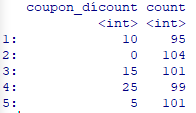
\includegraphics[width=0.4\linewidth]{graphics/5.3.1.png}
    \caption{Số lượng mặt hàng (count) theo từng loại chiết khấu (coupon\_discount)}
\end{figure}

Như đã thấy trên Hình, chỉ có 5 giá trị của coupon\_discount là : 0, 5, 10, 15, 25. Nhóm sẽ kiểm định xem, việc các mốc chiết khấu này sẽ ảnh hưởng như thế nào đến giá của các mặt hàng (order\_price) bằng phương pháp phân tích phương sai ANOVA mà nhóm đã thảo luận và đề xuất sử dụng. Dưới đây là phân tích phương sai ANOVA cho mẫu thống kê ( hàm phân tích đã được tích hợp sẵn trong R) :

\begin{figure}[!htbp]
    \centering
    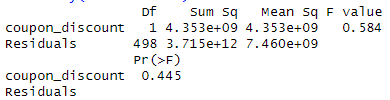
\includegraphics[width=0.4\linewidth]{graphics/5.3.2.png}
    \caption{Phân tích phương sai ANOVA xét sự ảnh hưởng của chiếc khấu (coupon\_discount) đến giá mặt hàng (order\_price)}
\end{figure}

Theo kết quả như hình trên, giá trị p-value (tức Pr(>F)) là 0.445 lớn hơn ngưỡng ý nghĩa phổ biến (0.05). Do đó, nhóm không đủ bằng chứng thống kê để kết luận rằng, chiết khấu (coupon\_discount) có ảnh hưởng đến giá trị đơn hàng (order\_price). Nói cách khác, sự khác biệt về giá trị đơn hàng giữa các nhóm chiết khấu có thể do yếu tố ngẫu nhiên.
Cũng trên bảng phân tích gọn (Hình 5.1),  số lượng mặt hàng (count) theo từng loại chiết khấu (coupon\_discount) cũng  không sai lệch quá lớn ( khoảng lệch giữa giá trị nhỏ nhất và lớn nhất theo giá trị lớn nhất chỉ là 8.654\%), điều này càng cũng cố tính chính xác của phương pháp.
nhóm có thể tính toán kích thước hiệu ứng (effect size) để đánh giá mức độ ảnh hưởng của một yếu tố (biến độc lập). Sử dụng Enhóm-squared (ɳ2) đo lường mức độ ảnh hưởng của coupon\_discount. Diễn dãy mở rộng (Field, 2013):

\begin{table}[ht]
    \centering
    \begin{tabular}{|c|c|}
    \hline
    \textbf{Khoảng giá trị ($\eta^2$)} & \textbf{Mức độ ảnh hưởng} \\ 
    \hline
    $\eta^2 < 0.01$ & Không đáng kể (negligible) \\ 
    \hline
    $0.01 \leq \eta^2 < 0.04$ & Nhỏ (small effect) \\ 
    \hline
    $0.04 \leq \eta^2 < 0.09$ & Vừa phải (moderate effect) \\ 
    \hline
    $\eta^2 \geq 0.09$ & Lớn (large effect) \\ 
    \hline
    \end{tabular}
    \caption{Bảng mô tả mức độ ảnh hưởng theo giá trị $\eta^2$}
    \label{table:effect_size}
\end{table}

Thực hiện trên R (hàm tích hợp sẵn) :
\begin{figure}[!htbp]
    \centering
    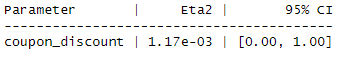
\includegraphics[width=0.6\linewidth]{graphics/5.3.3.png}
    \caption{Phân tích phương sai ANOVA xét sự ảnh hưởng của chiếc khấu (coupon\_discount) đến giá mặt hàng (order\_price)}
\end{figure}

Có thể thấy, giá trị ɳ2  của  coupon\_discount  tính trong thống kê rất nhỏ (0.001170329 <0.01), điều này nói lên được mức độ ảnh hưởng của chiết khấu (coupon\_discount) đến giá trị đơn hàng (order\_price) là không đáng kể.